\documentclass{article}
\usepackage{blindtext}
\usepackage[utf8]{inputenc}
\usepackage{amsmath,bm}
\usepackage{amstext}
\usepackage{amsfonts}
\usepackage{amsmath}
\usepackage{multirow}
\usepackage{enumerate}
\usepackage{xeCJK}
\setCJKmainfont{STKaiti}
\usepackage{algorithm}
\usepackage{algorithmic}
\renewcommand{\algorithmicrequire}{ \textbf{输入:}} %Use Input in the format of Algorithm
\renewcommand{\algorithmicensure}{ \textbf{输出:}} %UseOutput in the format of Algorithm
\usepackage{graphicx}

\title{Neural Network and Applications\\ 大作业一}
\author{陈轶洲 MF20330010}
\begin{document}
	\maketitle
	\numberwithin{equation}{section}
\section{设计方案}
本章将从三个方面介绍感知器神经网络的设计方案:
\begin{enumerate}[1)]
	\item 神经网络层设计:定义各层的结构,以及前向传播与反向传播计算方法;
	\item 网络结构设计:定义网络层数,各层激活函数,输入输出及各隐藏层规模,损失函数类型;
	\item 参数设计:定义训练数据集与测试数据集,以及训练轮次、学习率等超参数。
\end{enumerate}
\subsection{神经网络层设计}
本节将介绍三种隐藏层的设计,包括其前向传播与反向传播的计算方法。
\subsubsection{全连接层}
\begin{figure}[H]
	\centering
	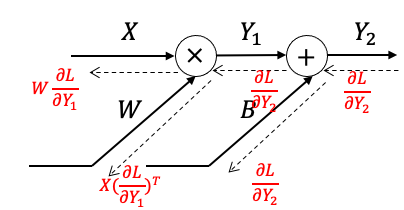
\includegraphics[scale=0.6]{FC.png}
\end{figure}
前向传播:
反向传播
\subsubsection{Relu层}

\subsubsection{Tanh层}

\section{编程实现方案}


\section{参数分析}


\section{实验结果展示}


\section{参考文献}
[1]https://zhuanlan.zhihu.com/p/47519999

\end{document}
